\chapter{Bezprzewodowe sieci czujnikowe}
Bezprzewodowe sieci czujnikowe są systemami składającymi się dużej liczby węzłów, z których każdy wyposażony w moduły umożliwiające gromadzenie, przetwarzanie oraz przesyłanie informacji \cite{Ilyas2004}, dzięki czemu możliwe staje się obserwowanie oraz reagowanie na zdarzenia występujące w objętym jej zasięgiem środowisku. Środowiskiem to może mieć charakter zarówno fizyczny, jak też i biologiczny, czy stanowić fragment systemu informatycznego. 
\cite{Sohraby2006}
Bezprzewodowa sieć czujnikowa składa się z czterech podstawowych elementów\cite{Karl2006}:
\begin{enumerate}
	\item Zestawu czujników rozmieszczonych na określonym obszarze
	\item Sieci łączącej te czujniki
	\item Co najmniej jednego węzła gromadzącego dane z pozostałych
	\item Węzłów lub zewnętrznej do sieci jednostki, której zadaniem jest przetworzenie zebranych danych
\end{enumerate}
W literaturze wyróżnia się również dodatkowo badane zjawisko oraz użytkownika chcącego uzyskać informacje na jego temat jako elementy składające się na architekturę sieci \cite{Tilak2002}.

Wartym odnotowania jest fakt, że przetwarzanie danych może się odbywać w samej sieci czujników, bez konieczności udziału zewnętrznych jednostek.

Sieci czujnikowe najczęściej same organizują swoją strukturę. Oznacza to, że hierarchia (lub jej brak) sieci oraz trasy pakietów są dynamicznie wypracowywane przez węzły sieci zgodnie z zaimplementowanymi protokołami.

Przed projektantami bezprzewodowych sieci czujnikowych stoi wiele wyzwań. W zależności od przeznaczenia oraz środowiska, w którym działa dana sieć wymagane jest inne podejście projektowe. Do pożądanych celów należą:
\paragraph{Niski koszt oraz małe rozmiary czujników}
Są one niezbędne w implementacjach bezprzewodowych sieci czujnikowych o szerokiej skali. W ramach kosztów należy uwzględnić zarówno koszt samej implementacji oraz wdrożenia, jak również koszty związane z utrzymaniem \cite{Howitt2006}.

\paragraph{Skalowalność architektury}
Bezprzewodowe sieci czujnikowe często działają w kontekście heterogenicznych aplikacji o zróżnicowanych wymaganiach. Przy takich warunkach konieczne staje się stworzenie elastycznej oraz skalowalnej architektury bezprzewodowej sieci czujnikowej. Dodatkową, niezbędną cechą takich sieci jest kompatybilność z istniejącymi już systemami \cite{Pakzad2008}.

\paragraph{Fuzja danych wraz z lokalnym ich przetwarzaniem}
W celu zmniejszenia narzutu komunikacyjnego oraz przesyłania nadmiarowych danych węzły sieci powinny przesyłać do węzła bazowego uprzednio odfiltrowane oraz przetworzone dane \cite{Wu2017, Abdelgawad2012}.

\paragraph{Optymalne korzystanie z dostępnych zasobów energetycznych}
Oszczędność energii węzłów jest konieczna do zapewnienia odpowiednio długiego czasu działania sieci. Sposób zużycia energii może zostać udoskonalony na poziomie każdej z warstw sieci czujników. Przykładami mogą być wydajne protokoły trasowania \cite{Pereira2016} oraz tryb oszczędzania energii w warstwie MAC \cite{Michael2006}.

\paragraph{Samoorganizacja sieci}
W bezprzewodowych sieciach czujnikowych topologia sieci jest dynamiczna. Spowodowane jest to przez usterki czujników, ich mobilność lub ich wyłączenie z powodu zużycia energii. Dzięki samoorganizacji liczba węzłów sieci może ulec zmianie bez wpływu na jej działanie \cite{Gungor2009}.

\paragraph{Adaptacja do warunków sieciowych}
Adaptacyjność sieci do zmiennych warunków medium bezprzewodowego jest niezbędna w zastosowaniach militarnych, przemysłowych oraz w monitoringu środowiska. Uzyskuje się ją dzięki wykorzystaniu odpowiednich algorytmów przetwarzania sygnałów oraz protokołów komunikacyjnych \cite{Gungor2009}.

\paragraph{Synchronizacja}
W bezprzewodowych sieciach czujnikowych samo zadanie zbierania danych oraz zebrane dane często podlegają ograniczeniom czasowym oraz są związane z opóźnieniami \cite{Alnuaimi2011}. Konieczna staje się więc synchronizacja węzłów sieci w czasie, aby spełnić wymagania narzucone na czas wykonywania operacji związanych z konkretną aplikacją sieci. Jednakże z powodu ograniczeń zasobów sieci oraz jej dynamicznej topologii nie mogą zostać zastosowane tradycyjne rozwiązanie zaprojektowane dla sieci przewodowych i bezprzewodowych. Konieczne staje się stworzenie protokołów synchronizacyjnych dedykowanych dla bezprzewodowych sieci czujnikowych \cite{Howitt2006}.

\paragraph{Tolerancja na awarie}
Punkt ten odnosi się do potrzeby bezawaryjnego przesłania odczytów do węzła bazowego, jak również poprawnego przesłania komend i zapytań do węzłów sieci oraz poprawnego ich wykonania. Spełnienie tych warunków wymaga wykorzystania odpowiednich protokołów weryfikujących oraz poprawiających przesyłane dane w każdej z warstw komunikacyjnych \cite{Kakamanshadi2015}.

\paragraph{Bezpieczeństwo}
W zależności od wymagań związanych z danym wdrożeniem konieczny jest różny poziom zabezpieczeń. Do przykładowych zabezpieczeń należą: kryptografia klucza publicznego, ochrona przed atakami DoS (denial of service), odporność na przejęcie węzła, wykrywanie włamań. Zastosowane rozwiązanie powinno brać pod uwagę ograniczone zasoby węzła \cite{Pathan2010}.

\bigskip

Przykładami zastosowań sieci czujnikowych są: gromadzenie danych, monitoring, telemetria medyczna \cite{Biradar2009}.

\section{Czujnik}
Czujnik z technicznego punktu widzenia jest urządzeniem, którego zadaniem jest zbieranie informacji o obiektach i procesach fizycznych wraz ze zmianami ich stanu \cite{Dargie2010}.

W celu stworzenia sieci czujników konieczne jest wcześniejsze zaprojektowanie i stworzenie pojedynczego węzła. Bardzo często narzucone są na nie dodatkowe ograniczenia: wielkość, pobór energii, koszt wytworzenia. Dodatkowo, węzły sieci muszą posiadać odpowiednie czujniki, moduły komunikacyjne oraz moc obliczeniową odpowiednią do ich obsłużenia. W książce \cite{Karl2006} architekturę sprzętową pojedynczego węzła rozbito na pięć komponentów:
\begin{enumerate}
	\item Sterownik - komponent odpowiedzialny za zbieranie danych z czujników oraz ich przetwarzanie. Ponadto decyduje on kiedy oraz gdzie wysłać te dane oraz steruje zachowaniem aktuatorów. Funkcje te realizuje dzięki wykonywaniu instrukcji zawartych w kodzie uprzednio napisanych programów. Sterownik można zrealizować wykorzystując różne architektury układów scalonych. Najczęściej używane są mikrokontrolery. Głównymi ich zaletami są łatwość w komunikacji z urządzeniami zewnętrznymi takimi jak np. czujniki, niski pobór energii (mogą zostać również przełączone w tryb uśpienia) oraz łatwa programowalność.
	\item Pamięć - komponent przechowujący programy oraz dane. Do przechowywania odczytów z czujników przed wysyłką lub przetworzeniem oraz odebranych pakietów wykorzystuje się pamięć RAM. Programy zapisywane są w pamięci ROM, EEPROM lub Flash. Pamięć Flash bywa również używana do przechowywania pomiarów w sytuacjach, gdy pamięć RAM okazuje się niewystarczająca lub w celu zapisu danych z pamięci RAM przed wyłączeniem czujnika.   
	\item Czujniki i aktuatory - urządzenia zbierające informacje o środowisku zewnętrznym oraz urządzenia wpływające na jego stan. Mogą to być między innymi czujniki wielkości elektrycznych, pola magnetycznego, wykrywacze fal radiowych, czujniki optyczne, elektrooptyczne, podczerwieni, lasery, radary, lokalizacyjne, fal sejsmicznych, badające parametry środowiskowe (pęd wiatru, temperaturę, wilgotność, ciśnienie), biochemiczne \cite{Sohraby2006}.
	\item Komunikacja - komponent odpowiedzialny za wysyłanie oraz odbieranie danych za pośrednictwem bezprzewodowego kanału komunikacyjnego. Najczęściej wykorzystywanym medium są fale radiowe - umożliwiają one wysyłanie danych na relatywnie długie dystanse przy małym zużyciu energii. 
	\item Zasilanie - najczęściej są to baterie lub ogniwa słoneczne
\end{enumerate}

\begin{figure}[H]
	\begin{center}
		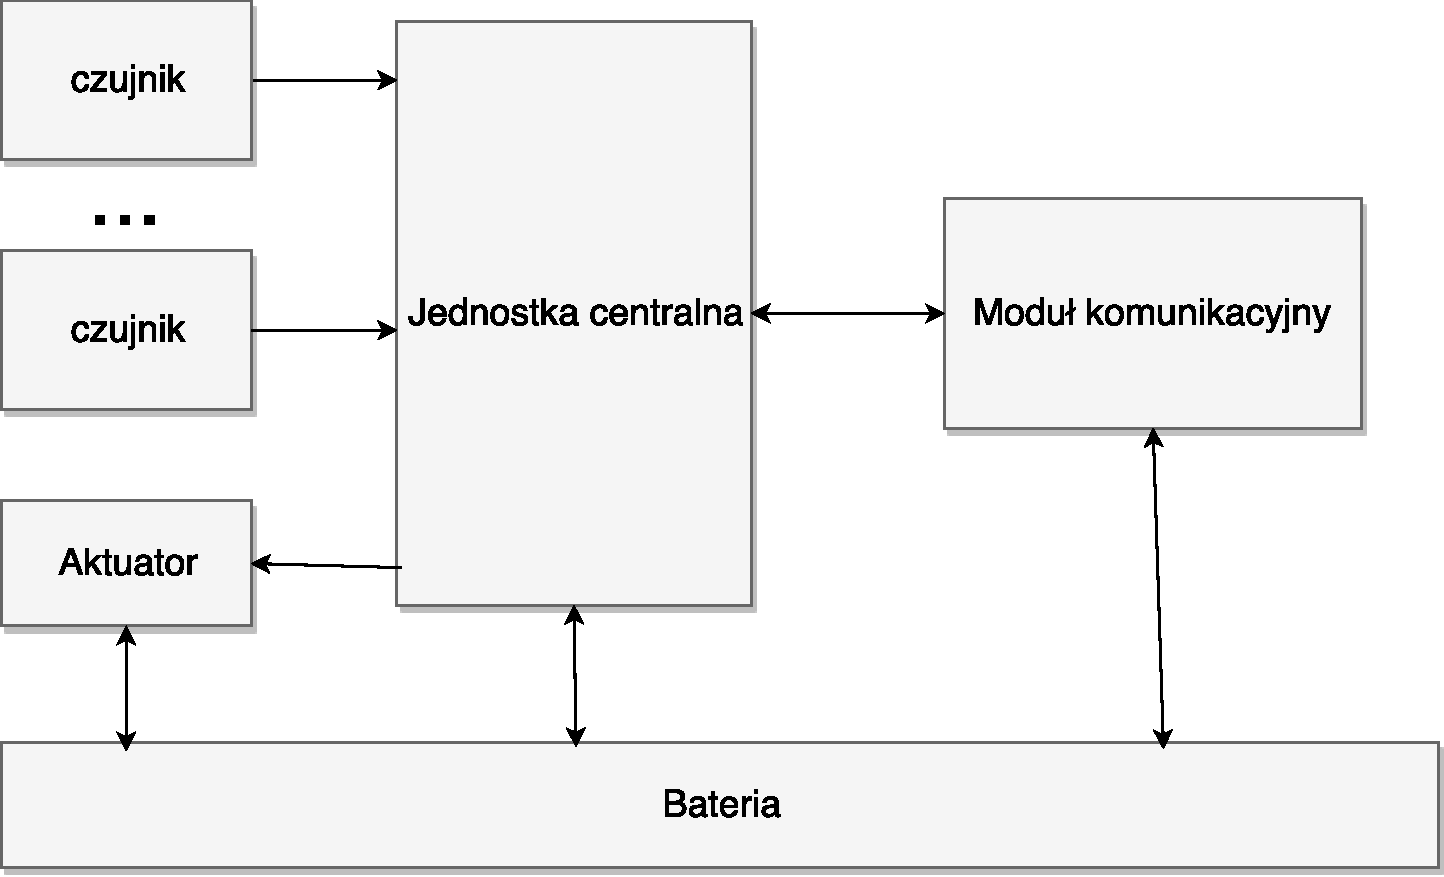
\includegraphics[scale=0.5]{\ImgPath/sensor_node.pdf}
	\end{center}
	\caption{Architektura węzła sieci czujnikowej}
\end{figure}

\section{Stos sieciowy bezprzewodowych sieci czujnikowych}

Bezprzewodowa sieć czujnikowa jest zbiorem wielofunkcyjnych węzłów czujnikowych zorganizowanych w sieć typu ad hoc. Wyróżnia się przy tym dwa główne schematy komunikacji. Pierwszym z nich odpowiada topologii gwiazdy, w której węzły komunikują się bezpośrednio z węzłem bazowym (komunikacja z jednym przeskokiem - single-hop). Drugi opisuje komunikację, w której pakiet danych przesyłany jest do węzła bazowego za pośrednictwem wielu węzłów z wykorzystaniem trasowania (komunikacja z wieloma przeskokami - multi-hop). Ten sposób pozwala na zmniejszenie zużycia energii, ponieważ zazwyczaj węzły rozmieszczone są w relatywnie małych odległościach od siebie (zagęszczenie może dochodzić nawet do 20 węzłów na $m^{3}$ \cite{Shih2001}).

Bezprzewodowe sieci czujnikowe posiadają jednak również pewne istotne różnice w stosunku do tradycyjnych sieci typu ad-hoc:
\begin{itemize}
\item Ograniczone zasoby energetyczne - często węzły sieci znajdują się w odległych, trudno dostępnych lokalizacjach, co uniemożliwia wymianę ich baterii. Wymusza to minimalizację zużycia energii, w celu uzyskania jak najdłuższego działania sieci.
\item Brak globalnych identyfikatorów węzłów sieci - w zastępstwie używana jest klasteryzacja.
\item Niedeterministyczne rozmieszczenie węzłów sieci - sieć organizuje się sama.
\end{itemize}

Stos protokołów bezprzewodowej sieci czujnikowej musi więc być zgodny z wymienionymi wcześniej cechami oraz osobliwościami tychże sieci. Okazuje się, że  stos protokołów sieciowych dla bezprzewodowych sieci czujnikowych przypomina tradycyjny model OSI (z wyłączeniem warstw prezentacji oraz sesji) \cite{Akyildiz2002.09}. Zawiera on następujące warstwy: aplikacji, transportową, sieciową, łącza danych oraz fizyczną.

\paragraph{Warstwa fizyczna}
odpowiedzialna jest za wybór częstotliwości, generowanie częstotliwości fali nośnej, wykrywanie i modulację sygnału. Przy projektowaniu warstwy fizycznej dla bezprzewodowych sieci czujnikowych zużycie energii jest istotniejszym czynnikiem od propagacji i zanikania fali. W ogólnym przypadku ilość energii potrzebna do transmisji sygnału na odległość $d$ jest proporcjonalna do $d^{n}$, gdzie $2 <= n < 4$. Wykładnik $n$ jest bliższy wartości $4$ dla nisko osadzonych w stosunku do poziomu ziemi anten \cite{Sohrabi1999} - co jest typowym przypadkiem dla sieci czujnikowych. W celu mitygacji tego problemu stosuje się komunikację wieloskokową (multi-hop) wykorzystując fakt gęstego rozmieszczenia węzłów sieci \cite{Akyildiz2002.09}.
Krytyczny dla bezawaryjnej komunikacji jest również wybór odpowiedniego rodzaju modulacji, takiego jak np. MFSK, OQPSK, MQAM czy UWB.

\paragraph{Warstwa łącza danych}
jest odpowiedzialna za multipleksowanie strumieni danych, wykrywanie ramek danych, dostęp do łącza (MAC) oraz detekcję błędów. Dla bezprzewodowych sieci czujnikowych tworzone są wyspecjalizowane protokoły MAC, które muszą spełniać dwa założenia \cite{Akyildiz2002.09, Demirkol2006}.
\begin{enumerate}
\item Stworzenie infrastruktury sieci, w tym utworzenie połączeń komunikacyjnych pomiędzy tysiącami węzłów.
\item Umożliwienie wydajnego współdzielenia zasobów komunikacyjnych pomiędzy wszystkimi węzłami sieci.
\end{enumerate}
Dodatkowo należy wziąć pod uwagę wysoką decentralizację sieci oraz jej dynamicznie zmienną topologię. Przykładami takich dedykowanych protokołów MAC mogą być S-MAC \cite{Ye2002}, WiseMAC \cite{Hoiydi2004}, CSMA \cite{Althobaiti2015} czy też TDMA \cite{Althobaiti2015}.

\paragraph{Warstwa sieciowa}
Podobnie, jak w przypadku protokołów warstwy łącza danych również i dla tej warstwy zostały stworzone dedykowane protokoły trasowania. Trasowanie w bezprzewodowych sieciach czujnikowych zostało szerzej opisane w podrozdziale \ref{routing}.

\paragraph{Warstwa transportowa}
Potrzeba wykorzystania warstwy transportowej pojawia się w momencie, gdy planowany jest dostęp do sieci czujnikowej z sieci Internet lub innej zewnętrznej sieci. Protokoły transportowe dla bezprzewodowych sieci czujnikowych powinny spełnić szereg warunków:
\begin{itemize}
\item Kontrola nad przeciążeniem sieci
\item Uproszczenie inicjowania połączeń w celu zwiększenia przepustowości sieci oraz ograniczenia opóźnień
\item Minimalizacja utraty pakietów
\item Zapewnienie każdemu węzłowi sieci takiej samej przepustowości łącza
\item Komunikacja z pozostałymi warstwami sieci - mogą one dostarczyć cennych informacji protokołowi komunikacyjnemu, np. dotyczących nieudanego trasowania.
\end{itemize}
Tradycyjnie używane protokoły takie jak TCP i UDP nie są odpowiednie dla bezprzewodowych sieci czujnikowych \cite{Fahmy2016-2}. Do dedykowanych protokołów należą m. in. CODA \cite{Wan2003}, ESRT \cite{Akan2005}, RMST \cite{Stann2003} czy PSFQ \cite{Wan2002}.

\paragraph{Warstwa aplikacji}
stanowi abstrakcję nad fizyczną topologią bezprzewodowej sieci czujników na potrzeby aplikacji. Dodatkowo zapewnia ona użytkownikom interfejs do interakcji ze światem fizycznym za pośrednictwem sieci czujników. Wyróżnia się kilka kategorii protokołów warstwy aplikacji \cite{Akyildiz2010}:
\begin{itemize}
\item Kompresja danych - stosowana jest za każdym razem, gdy dany węzeł uzyskał nową informację do przesłania. Dzięki kompresji możliwa jest minimalizacja wielkości przesyłanych pakietów danych. Najczęściej używanym rodzajem kompresji w bezprzewodowych sieciach czujnikowych jest kompresja bezstratna. Ze względu na ograniczoną pamięć oraz moc obliczeniową węzłów nie można zastosować standardowych algorytmów takich jak LZW, czy gzip. Do specjalnie zaprojektowanych na potrzeby bezprzewodowych sieci czujnikowych algorytmów należą Sensor–LZW \cite{Sadler2006} oraz DSC \cite{Slepian1973, Wyner1976}.
\item Przetwarzanie zapytań - dostęp do żądanych danych zapewnia użytkownikowi węzeł bazowy za pośrednictwem zapytań. Odpowiedzią sieci mogą być zarówno surowe dane przesłane do stacji bazowej, ale często spotykane są również bardziej wyrafinowane schematy przetwarzania zapytań uwzględniające konserwację energii. Z tego punktu widzenia, bezprzewodową sieć czujników można postrzegać jako rozproszoną bazę danych \cite{Madden2002}.
\item Zarządzanie siecią - dynamiczna natura bezprzewodowych sieci czujnikowych wymaga monitorowania oraz zarządzania jej częściami składowymi. Z potrzeby tej wynikło stworzenie dedykowanych narzędzi administracyjnych, takich jak MANNA \cite{Ruiz2003} czy SNMS \cite{Tolle2005}.
\end{itemize}

\section{Trasowanie w WSN} \label{routing}
Bezprzewodowe sieci czujnikowe mają wiele wspólnego z sieciami przewodowymi i ad-hoc, jednakże wykazują również swoje własne, unikatowe cechy oraz związane z nimi wyzwania.
Jedną z takich cech jest różnorodna gęstość sieci oraz liczby węzłów. Sieci czujnikowe mogą składać się z kilkuset do kilku tysięcy węzłów, rozmieszczonych w sposób losowy o różnorodnym zagęszczeniu. Zachowanie tych węzłów jest dynamiczne, jako że do ich zadań oprócz zbierania danych oraz przesyłania pakietów należy również oszczędzanie własnej energii. Dodatkowo duży wpływ na jakość połączenia mają wysokie poziomy szumu oraz interferencja.
Istotnym wyzwaniem związanym z sieciami czujników jest również model danych oraz ich przepływu, który różni się w zależności od konkretnego rozwiązania, w którym sieć jest wykorzystywana. Węzły sieci mogą cyklicznie wysyłać do stacji bazowej próbkę danych. W modelu zdarzeniowym węzeł sieci wysyła pakiet po wystąpieniu określonego zjawiska. Istnieją również implementacje wymagające od węzłów sieci przetwarzania oraz agregacji danych przez węzeł, przed ich wysyłką, czy takie, które wymagają komunikacji dwukierunkowej pomiędzy węzłami a stacją bazową.

%Więcej wyzwań z Routing Protocols in Wireless Sensor Networks –
%A Survey

Taka różnorodność modeli przepływu danych oraz innych wyzwań wymagają zastosowania odpowiednio zoptymalizowanych algorytmów trasowania \cite{Abdullah2014, Sohraby2006}.

Z powodu różnych potrzeb odnośnie trasowania pakietów zaproponowany został szereg metryk dotyczących zasobów sieci. Celem protokołów trasowania jest optymalizacja ich wykorzystania. \cite{Dargie2010, Biradar2009}.
\begin{itemize}
 \item Minimalizacja ścieżki pakietu do węzła bazowego
 \item Minimalizacja energii zużytej na wysłanie pakietu
 \item Maksymalizacja czasu, po którym następuje podział sieci
 \item Minimalizacja wariancji poziomów energii węzłów
\end{itemize}

\subsection{Flood}\label{subsec:flood}
Węzeł wysyłający pakiet rozgłasza go do najbliższych sąsiadów, którzy z kolei powtarzają ten krok, aż pakiet dotrze do wszystkich węzłów sieci lub osiągnie maksymalną liczbę skoków.
W przypadku tego algorytmu, jeżeli istnieje droga łącząca źródło pakietu z celem, to cel z pewnością go otrzyma.
Zaletą tego algorytmu jest jego prostota. Do wad natomiast zalicza się duży ruch pakietów w sieci. W celu jego ograniczenia oraz zapewnienia aby pakiet nie był wysyłany w nieskończoność stosowane są dwa mechanizmy \cite{Dargie2010}:
\begin{itemize}
	\item maksymalna liczba przeskoków pakietu
	\item numery sekwencji pakietów - pakiety otrzymują kolejne numery, które wraz z adresem węzła wysyłającego umożliwiają jego identyfikację. Dzięki temu węzły mogą przechowywać historię otrzymanych (oraz rozgłoszonych dalej pakietów) i w momencie w którym taki pakiet ponownie otrzymają - go odrzucić.
\end{itemize}

Mechanizmy te jednakże nie rozwiązują następujących problemów występujących w protokole Flood \cite{Dargie2010}:
\begin{itemize}
	\item Implozja - węzeł, który otrzymał pakiet rozgłasza go do swoich sąsiednich węzłów niezależnie od tego, czy otrzymały one już ten pakiet od innego węzła. Prowadzi to do niepotrzebnego zużycia zasobów. %Dorzucić obrazek
	\item Redundancję geograficzną - pakiety wysyłane przez węzły monitorujące pokrywające się obszary są traktowane jako kompletnie od siebie różne (brak fuzji danych), co prowadzi do marnowania zasobów (ta sama informacji wysyłana jest wielokrotnie). %Dorzucić obrazek
	\item Nieuwzględnianie zasobów węzła - ze względu na swoją prostotę algorytm nie bierze pod uwagę aktualnych zasobów węzła sieci, takich jak dostępna pamięć, czy energia węzła.
\end{itemize}
\subsection{SPIN}
Protokół SPIN (Sensor Protocols for Information via Negotiation) jest rodziną protokołów trasowania typu płaskiego. Do rozsyłania informacji po sieci wykorzystują one negocjację. Do ich przeprowadzenia używają pakietów zawierających metadane, które opisują przesyłane wiadomości. Dzięki temu możliwe jest wyeliminowanie redundancji transmisji występujące w protokołach typu Flood \cite{Chaudhary2015}.

Projekt SPIN wyrósł z protokołu Flood. Twórcy zauważyli trzy podstawowe problemy w tego typu podejściu, które opisane zostały w podrozdziale \ref{subsec:flood}

Innowacjami w stosunku do protokołu Flood są negocjacja oraz adaptacja w zależności od zasobów.

\paragraph{Negocjacja} W celu rozwiązania problemów związanych z implozją oraz przenikaniem się monitorowanych obszarów, przed wysłaniem pakietu węzły negocjują między sobą. Do negocjacji wykorzystywane są dodatkowe informacje o pakietach - meta-dane. 
Meta-dane wykorzystywane są do precyzyjnego opisu danych zbieranych przez czujniki. Rozmiar w bajtach meta-danych musi być mniejszy od rozmiaru samego pakietu z danymi, aby rozwiązanie miało sens.
Sam protokół nie narzuca tego co meta-dane powinny zawierać. Jest to zależne od konkretnego rozwiązania oraz implementacji. Może to być np. identyfikator węzła, współrzędne geograficzne, itd. Specyfikacja, przechowywanie oraz przetwarzanie meta-danych wykracza poza algorytm SPIN.
W protokole SPIN węzły komunikują się za pomocą trzech rodzajów pakietów:
\begin{itemize}
	\item ADV - ogłoszenie nowych danych. Jest to pakiet zawierający meta-dane. Ogłasza on węzłom pojawienie się nowych danych
	\item REQ - zgłoszenie zamówienia na dany pakiet z danymi. Węzeł, który chce otrzymać konkretny pakiet wysyła wiadomość z jego meta-danymi (tymi, które otrzymał w ADV)
	\item DATA - pakiet zawierający właściwe dane z czujnika wraz z meta-danymi
\end{itemize}
Przebieg negocjacji ilustruje rysunek \ref{fig:spin}.
\begin{figure}[H]
	\label{fig:spin}
	\begin{center}
		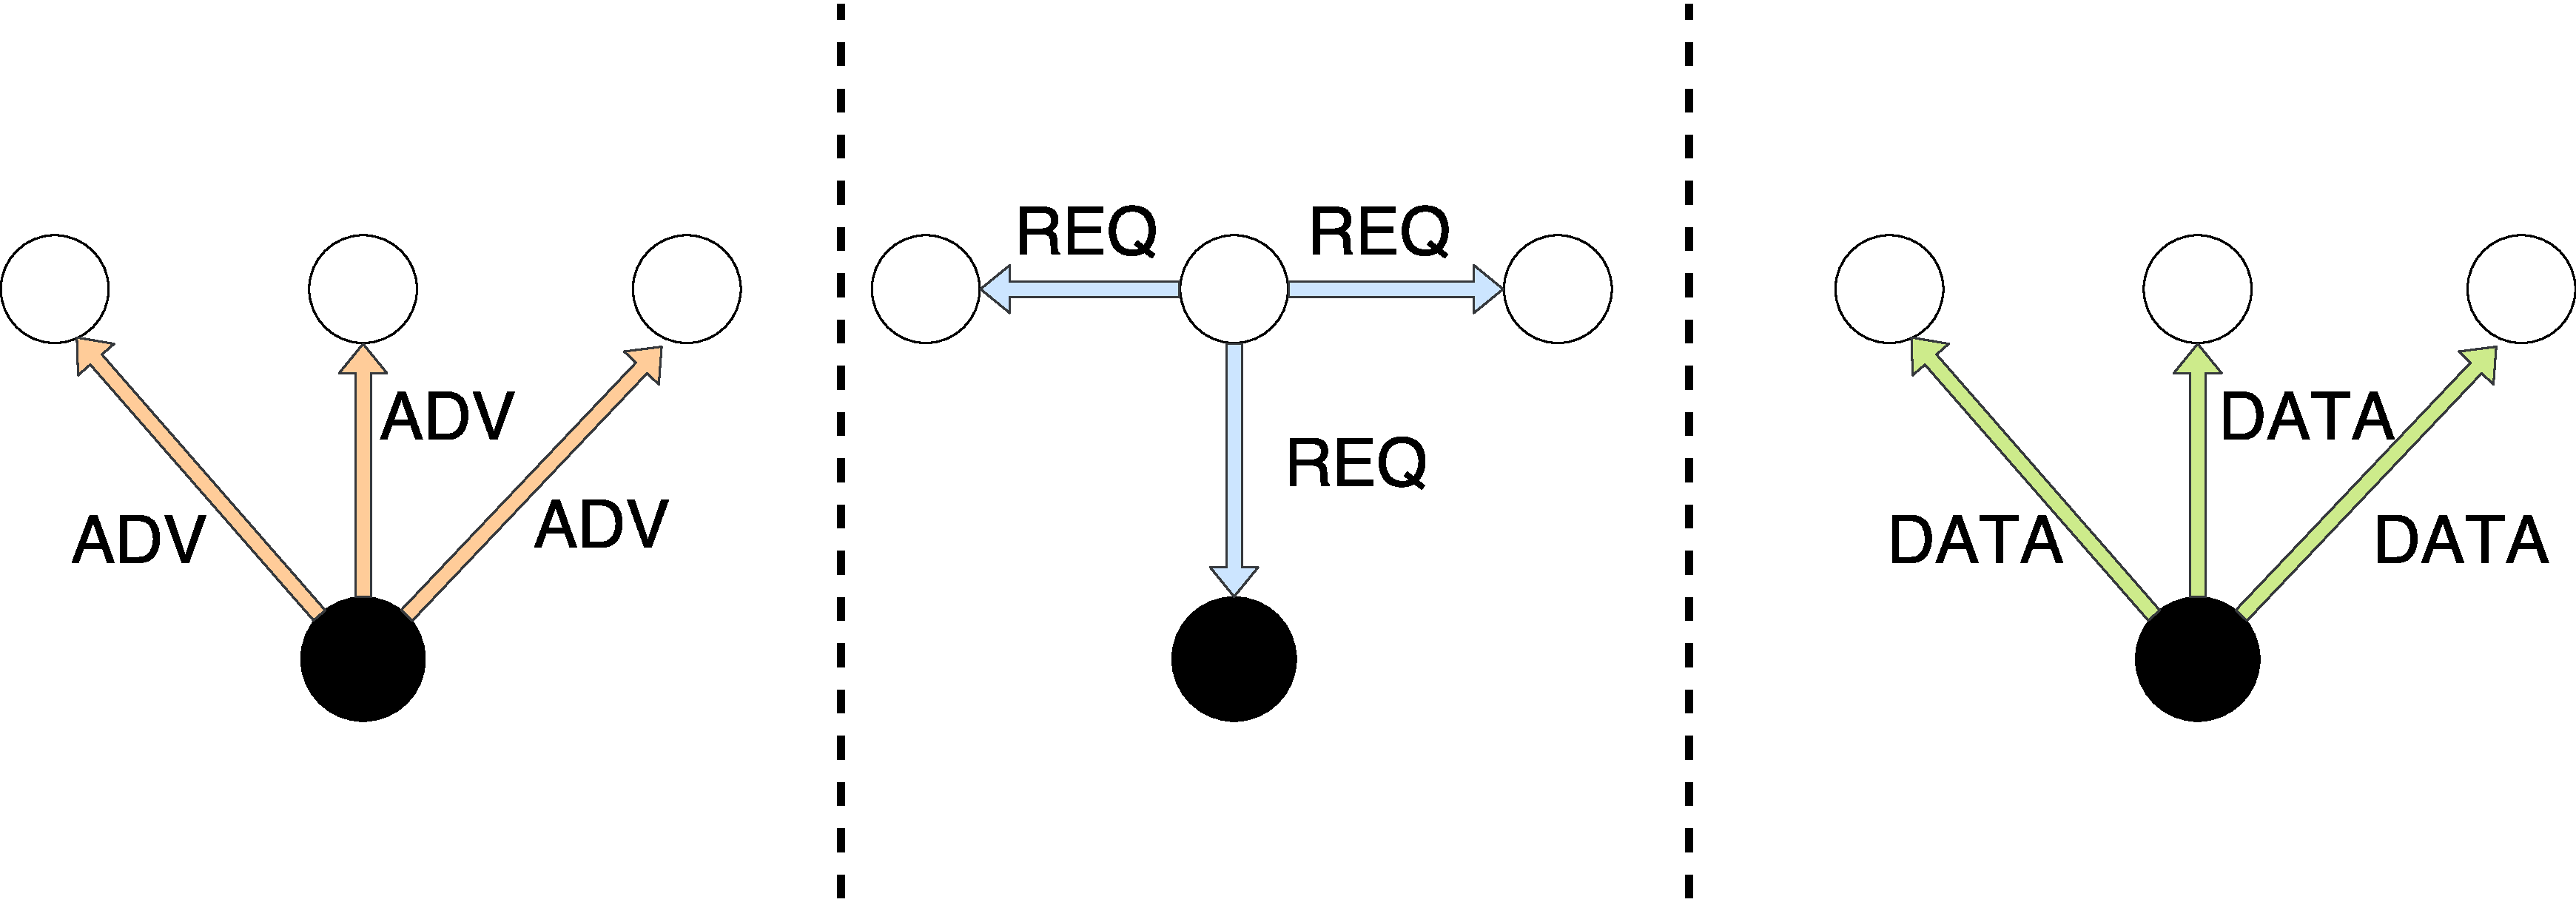
\includegraphics[scale=0.25]{\ImgPath/protocols/spin.pdf}
	\end{center}
	\caption{Przebieg negocjacji w protokole SPIN}
\end{figure}

Jako, że pakiety ADV i REQ zawierają tylko meta-dane, są one tańsze do wysłania niż DATA.

W skład rodziny algorytmów SPIN wchodzą cztery protokoły: SPIN-PP, SPIN-EC, SPIN-BC, SPIN-RL. Jako, że protokoły SPIN-PP oraz SPIN-EC nie przeznaczone są dla sieci point-to-point, opisane zostaną dwa pozostałe protokoły \cite{Dargie2010, Kulik2002}.

Protokół zaczyna się od wysłania pakietu ADV przez węzeł, który posiada nowe dane, które chce rozpropagować w sieci. Węzły sąsiednie, które otrzymały wiadomość ADV, sprawdzają czy otrzymały już takie dane. Jeśli reklamowane dane są dla nich nowe, wysyłają one wiadomość REQ z powrotem do nadawcy. Węzeł inicjujący negocjację po otrzymaniu wiadomości REQ wysyła dane w pakiecie DATA

\subparagraph{SPIN-BC}
W tym wariancie wykorzystany jest fakt, że węzły współdzielą medium komunikacyjne. Komunikacja pomiędzy dwoma węzłami może zostać ''podsłuchana'' przez węzły znajdujące się w zasięgu. Wszystkie pakiety wysyłane są w trybie rozgłoszeniowym, jako że dla sieci bezprzewodowej nie wiąże się to z dodatkowym kosztem.

Wiadomość ADV jest rozgłaszana do wszystkich sąsiednich węzłów. Jednakże przed wysłaniem wiadomości REQ węzły czekają przez losowy okres. Jeżeli węzeł przechwycił wiadmość REQ dotyczącą tych samych danych, których i on potrzebuje, anuluje on wysyłkę swojej wiadomości REQ (nie jest potrzebna, redukuje to koszty). Pozwala to również na uniknięcie kolizji. Po otrzymaniu REQ węzeł wysyła pakiet DATA do kanału rozgłoszeniowego. Pakiet DATA jet wysyłany tylko raz, następujące po nim wiadomości REQ dotyczące tych samych danych są ignorowane.
\subparagraph{SPIN-RL}
SPIN-RL jest przystosowaniem SPIN-BC do warunków komunikacji stratnej. Każdy węzeł przechowuje listę wiadomości ADV i jeśli nie otrzyma on danych w odpowiednim czasie, to ponawia on wysyłkę zapytania o dane (REQ). Odbiorca jest losowany z listy węzłów które wysłały ogłoszenie o tych samych danych.
Po wysyłce pakietu DATA musi upłynąć pewien odstęp czasowy przed ponowną wysyłką.

%Zakończenie
Zgodnie z badaniami opisanymi w artykule \cite{Kulik2002} protokoły SPIN są w stanie dostarczyć 60\% więcej danych w sieciach point-to-point i 80\% więcej danych w sieciach rozgłoszeniowych niż tradycyjne rozwiązania.  
\subsection{LEACH} \label{subsec:leach}
LEACH jest protokołem typu hierarchicznego, który wykorzystuje dwa poziomy grupowania węzłów. Pakiety trasowane są od czujników do lokalnych węzłów bazowych i od lokalnych węzłów bazowych do stacji bazowej \cite{Yu2006}.
Węzły same organizują się w klastry, w których jeden węzeł pełni funkcję lokalnego węzła bazowego - nazywany jest on również Cluster Head. W przeciwieństwie do konwencjonalnych algorytmów lokalne węzły bazowe nie są wybierane a priori. Wybierane są rotacyjnie w sposób losowy, tak aby równomiernie rozłożyć zużycie energii oraz wybierać węzły z możliwie jak największą energią. Dodatkowo LEACH wykorzystuje fuzję danych w celu skompresowania ich ilości przesyłanych z klastra do stacji bazowej \cite{Akkaya2005, Heinzelman00}.

Działanie algorytmu podzielone jest na rundy. Każda runda składa się z fazy konfiguracyjnej, po której następuje faza stabilnego działania sieci. W fazie początkowej każdy węzeł decyduje o tym czy ma zostać lokalnym węzłem bazowym w aktualnej rundzie. Decyzja ta opiera się na zadanej przez użytkownika liczbie lokalnych węzłów bazowych w sieci (wyrażonej jako procent liczby wszystkich węzłów sieci) oraz na fakcie uprzedniego bycia lokalnym węzłem bazowym.
Algorytm ten przebiega w sposób następujący:
\begin{enumerate}
	\item Węzeł n losuje liczbę z zakresu od 0 do 1
	\item Obliczany jest próg wyrażony poniższym wzorem
	\[T(n) = \begin{dcases} 
      \frac{P}{1-P*(r\:mod\frac{1}{P})} & n \in G \\
      0 & n \not\in G \\
   \end{dcases}
	\]
	, gdzie P - procent sieci, którą powinny stanowić lokalne węzły bazowe,
	r - numer aktualnej rundy
	G - zbiór węzłów, które nie były lokalnymi węzłami bazowymi przez ostatnie $\frac{1}{P}$ rund.
	\item Jeżeli wylosowana liczba jest mniejsza od progu $T(n)$, to węzeł zostaje lokalnym węzłem bazowym.
\end{enumerate}
Taki wybór lokalnych węzłów bazowych gwarantuje, że każdy węzeł sieci zostanie nim w ciągu $\frac{1}{P}$ rund. Wszystkie węzły, które zostały wybrane jako lokalne węzły bazowe w pierwszej rundzie (o numerze 0) nie zostaną nimi przez kolejnych $\frac{1}{P}$ rund. Przez kolejne rundy wartość progu $T(n)$ rośnie. Funkcja została zaprojektowana w ten sposób, aby wraz ze zmniejszaniem się liczby węzłów, które mogą zostać potencjalnie wybrane na lokalne węzły bazowe prawdopodobieństwo ich wyboru rosło. Po $\frac{1}{P}$ rundach próg $T(n)$ wraca do stanu początkowego, tym samym rozpoczynając ponownie opisany cykl.
Powyższy algorytm zakłada, że wszystkie węzły są homogeniczne pod względem początkowej ilości energii oraz jej zużywania.

Węzeł, który został wybrany na lokalny węzeł bazowy ogłasza ten fakt  pozostałym węzłom. Wykorzystywany jest przy tym protokół MAC CSMA. W tym czasie pozostałe węzły sieci muszą mieć włączone odbiorniki radiowe. Po zakończeniu tej fazy każdy z węzłów sieci nie będący lokalnym węzłem bazowym dokonuje decyzji, do którego klastra będzie należeć. Wybrany zostaje ten klaster, od którego zostało otrzymane ogłoszenie o największym wskaźniku mocy odebranego sygnału (z ang. RSSI - Received Signal Strength Indication). Dzięki tymi wybrany zostaje lokalny węzeł bazowy, z którym komunikacja jest najmniej kosztowna energetycznie.

Po dokonaniu wyborów klastrów przez węzły muszą one ów wybór zakomunikować lokalnym węzłom bazowym. Wysyłają więc one pakiet informujący o dołączeniu do klastra lokalnym węzłom bazowym (również z wykorzystaniem protokoły MAC CSMA).

Po otrzymaniu informacji zwrotnej od węzłów, lokalne węzły bazowe tworzą harmonogramy TDMA na podstawie liczby węzłów w klastrze. Wykorzystanie TDMA umożliwia zredukowanie kolizji podczas komunikacji \cite{Ilyas2004, Ergen2010}. Z pozostałego czasu rundy przeznaczonego na fazę stabilną wydzielane są dla każdego węzła przedziały czasowe, podczas których mogą one wysłać swoje pakiety z danymi do lokalnego węzła bazowego \cite{Cionca2008}. Harmonogram zostaje rozgłoszony do wszystkich węzłów w klastrze.

Po utworzeniu klastrów oraz harmonogramów TDMA, następuje faza stabilnego działania sieci, podczas której węzły przesyłają zebrane dane do lokalnych węzłów bazowych. Każdy węzeł transmituje pakiety w wyznaczonym dla niego przedziale czasowym. Transmisja odbywa się przy użyciu minimalnej energii, tak aby pakiet mógł dotrzeć do lokalnego węzła bazowego. Pozostałe węzły w klastrze (nie biorące udziału w transmisji) mogą w tym czasie wyłączyć odbiorniki radiowe w celu oszczędzania energii. Po otrzymaniu pakietu z danymi, lokalny węzeł bazowy przetwarza go oraz agreguje zgodnie z zaimplementowanymi regułami. Sposób kompresji oraz agregacji sygnałów jest dostosowywany do specyfiki danych zbieranych przez sieć (np. dane o temperaturze mogą zostać uśrednione w pewnym przedziale czasu). Po zebraniu danych lokalny węzeł bazowy przesyła je w pakiecie do stacji bazowej, po czym następuje nowa runda \cite{Yadav2014}.
\begin{figure}[H]
	\begin{center}
		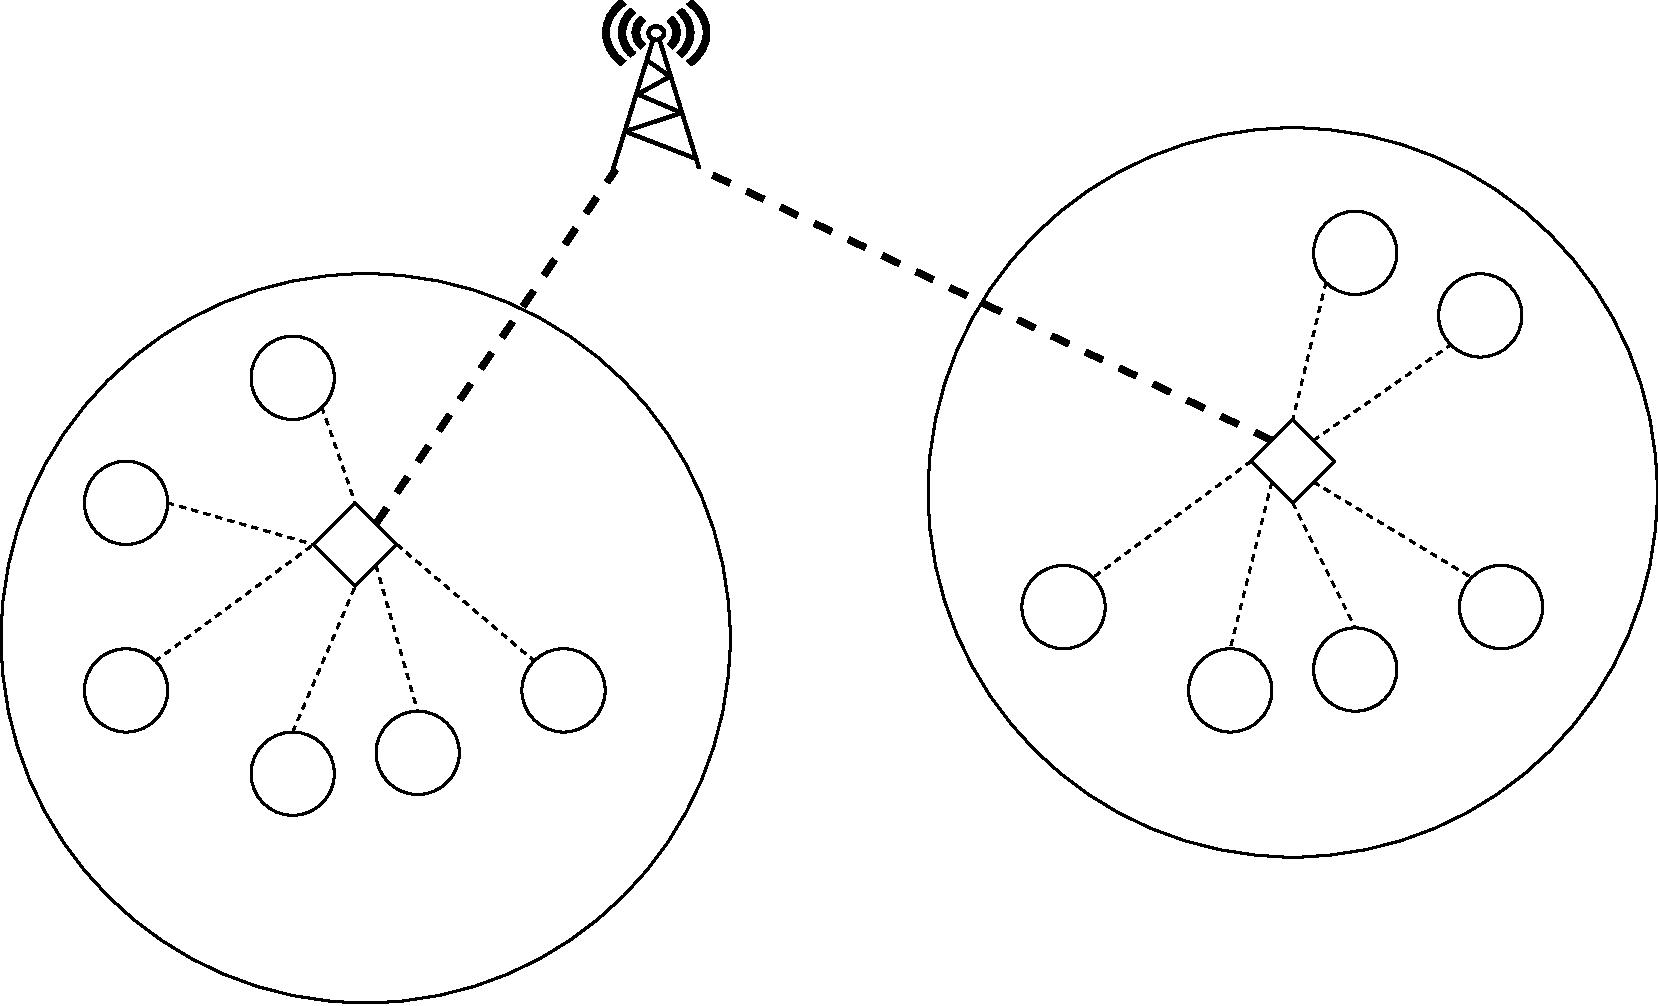
\includegraphics[scale=0.3]{\ImgPath/protocols/leach.pdf}
	\end{center}
	\caption{LEACH}
\end{figure}
\paragraph{ALEACH (Advanced LEACH)} \label{para:aleach}
ALEACH zmienia sposób wyboru lokalnego węzła bazowego. Nowy sposób obliczania progu $T(n)$ opiera się na nowych parametrach nazwanych prawdopodobieństwem aktualnego stanu oraz globalnym prawdopodobieństwie \cite{Ali2008}.

\[
	T(n) = G_{p} + CS_{p}
\]

Prawdopodobieństwo aktualnego stanu ($CS_{p}$) wyrażone jest poniższym wzorem \cite{Ali2008}.
\[
	CS_{p} = \frac{E_{aktualne}}{E_{n-max}}*\frac{K}{N}
\]
Gdzie $E_{aktualne}$ oznacza aktualną energię węzła, $E_{n-max}$ stanowi początkową energię sieci, $K$ spodziewaną liczbę lokalnych węzłów bazowych w rundzie, a $N$ liczbę wszystkich węzłów sieci. Im większa energia pozostała w danym węźle, tym większe jest prawdopodobieństwo, że zostanie on lokalnym węzłem bazowym.

Prawdopodobieństwo globalne natomiast liczone jest zgodnie ze wzorem \cite{Ali2008}:
\[
	G_{p} = \frac{K}{N - K * (r \:mod \frac{N}{K})}
\]

Pozostała część algorytmu jest taka sama jak w LEACH. Dzięki uwzględnieniu podczas wyboru lokalnego węzła bazowego jego aktualnej energii algorytm ten pozwala na wydłużenie życia sieci w stosunku do LEACH \cite{Singh2017}.
\paragraph{LEACH DCHS (LEACH-Deterministic Cluster Head Selection)}
Celem tego wariantu protokołu LEACH, tak samo jak w przypadku ALEACH, jest wydłużenie działania sieci czujników. Efekt ten został uzyskany dzięki modyfikacji progu $T(n)$ \cite{Handy2002, Singh2017}.
 \[
	T(n) =  \frac{P}{1 - P * (r \:mod \frac{1}{P})} * \left[\frac{E_{n_{aktualne}}}{E_{max}} + \left(r_{s} \backslash \frac{1}{p}\right)\left(1 - \frac{E_{n_{aktualne}}}{E_{max}}\right)\right]
\]

Włączenie aktualnego poziomu energii węzła do wzoru umożliwia zwiększenie prawdopodobieństwa wyboru węzła o większej energii na lokalny węzeł bazowy. Dodatkowo wraz z upływem czasu zwiększa się prawdopodobieństwo wyboru węzłów, które najdłużej nie pełniły tej funkcji. Odpowiada za to fragment $r_{s} \backlash \frac{1}{p}$.